\documentclass[10pt, compress]{beamer}

\usetheme{m}

\usepackage{booktabs}
\usepackage[scale=2]{ccicons}
\usepackage{minted}
\usepackage{graphicx} %package to manage images

\def\ab{\mbox{\boldmath $a$}}
\def\bb{\mbox{\boldmath $b$}}
\def\cb{\mbox{\boldmath $c$}}
\def\db{\mbox{\boldmath $d$}}
\def\eb{\mbox{\boldmath $e$}}
\def\fb{\mbox{\boldmath $f$}}
\def\gb{\mbox{\boldmath $g$}}
\def\hb{\mbox{\boldmath $h$}}
\def\ib{\mbox{\boldmath $i$}}
\def\jb{\mbox{\boldmath $j$}}
\def\kb{\mbox{\boldmath $k$}}
\def\lb{\mbox{\boldmath $l$}}
\def\mb{\mbox{\boldmath $m$}}
\def\nb{\mbox{\boldmath $n$}}
\def\ob{\mbox{\boldmath $o$}}
\def\pb{\mbox{\boldmath $p$}}
\def\qb{\mbox{\boldmath $q$}}
\def\rb{\mbox{\boldmath $r$}}
\def\sb{\mbox{\boldmath $s$}}
\def\tb{\mbox{\boldmath $t$}}
\def\ub{\mbox{\boldmath $u$}}
\def\vb{\mbox{\boldmath $v$}}
\def\wb{\mbox{\boldmath $w$}}
\def\xb{\mbox{\boldmath $x$}}
\def\yb{\mbox{\boldmath $y$}}
\def\zb{\mbox{\boldmath $z$}}

\def\Ab{\mbox{\boldmath $A$}}
\def\Bb{\mbox{\boldmath $B$}}
\def\Cb{\mbox{\boldmath $C$}}
\def\Db{\mbox{\boldmath $D$}}
\def\Eb{\mbox{\boldmath $E$}}
\def\Fb{\mbox{\boldmath $F$}}
\def\Gb{\mbox{\boldmath $G$}}
\def\Hb{\mbox{\boldmath $H$}}
\def\Ib{\mbox{\boldmath $I$}}
\def\Jb{\mbox{\boldmath $J$}}
\def\Kb{\mbox{\boldmath $K$}}
\def\Lb{\mbox{\boldmath $L$}}
\def\Mb{\mbox{\boldmath $M$}}
\def\Nb{\mbox{\boldmath $N$}}
\def\Ob{\mbox{\boldmath $O$}}
\def\Pb{\mbox{\boldmath $P$}}
\def\Qb{\mbox{\boldmath $Q$}}
\def\Rb{\mbox{\boldmath $R$}}
\def\Sb{\mbox{\boldmath $S$}}
\def\Tb{\mbox{\boldmath $T$}}
\def\Ub{\mbox{\boldmath $U$}}
\def\Vb{\mbox{\boldmath $V$}}
\def\Wb{\mbox{\boldmath $W$}}
\def\Xb{\mbox{\boldmath $X$}}
\def\Yb{\mbox{\boldmath $Y$}}
\def\Zb{\mbox{\boldmath $Z$}}

\def\zerob{\mbox{\boldmath $0$}}


\usepackage{tikz}

\usetikzlibrary{scopes}
%\documentclass[tikz, border=5pt]{standalone}
\usetikzlibrary{calc}
\usetikzlibrary{patterns}
\usepackage{tkz-euclide}
\usetkzobj{all}

\usemintedstyle{trac}

\usefonttheme[onlymath]{serif}

\newcommand\der{{\rm d}}

\title{Robot Inverse Kinematics using SQP method}
\subtitle{}
\date{\today}
\author{Xiaoqian Mu, Yuechuan Xue}
\institute{Iowa State University}

\begin{document}

\maketitle

\begin{frame}[fragile]{Robot}
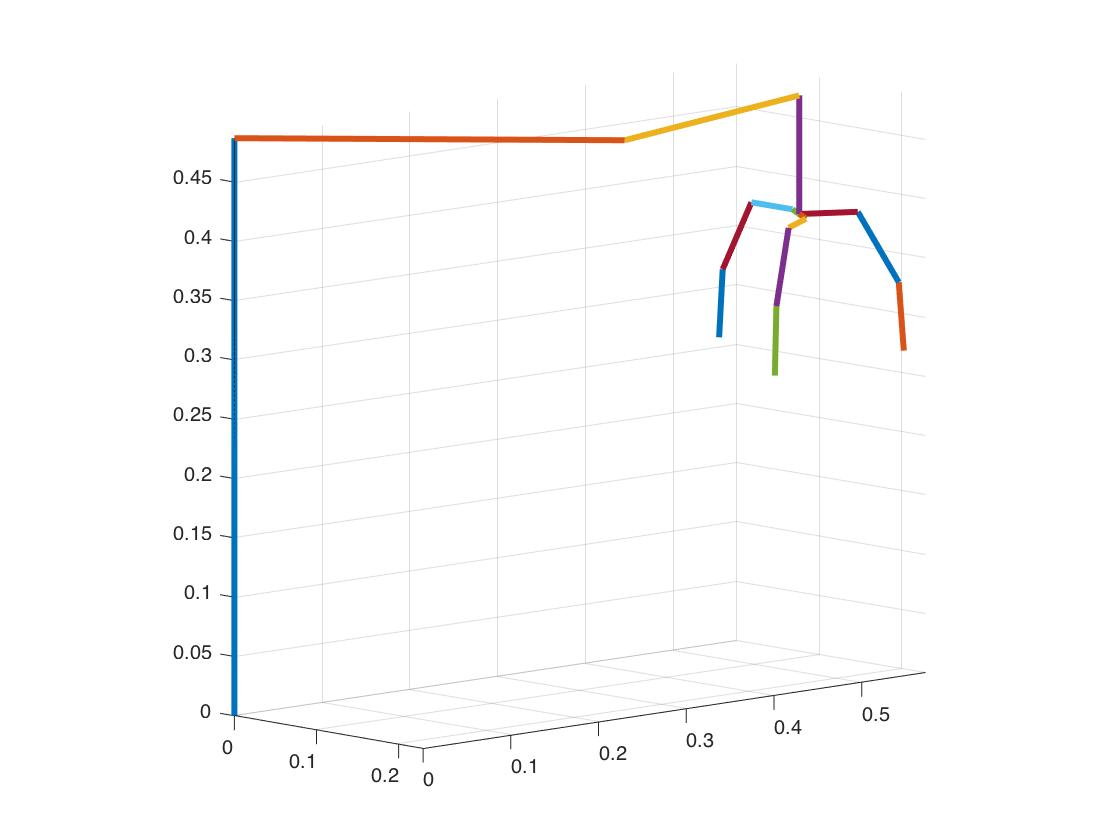
\includegraphics[width=6cm, height=4cm]{robot-matlab-config.jpg}
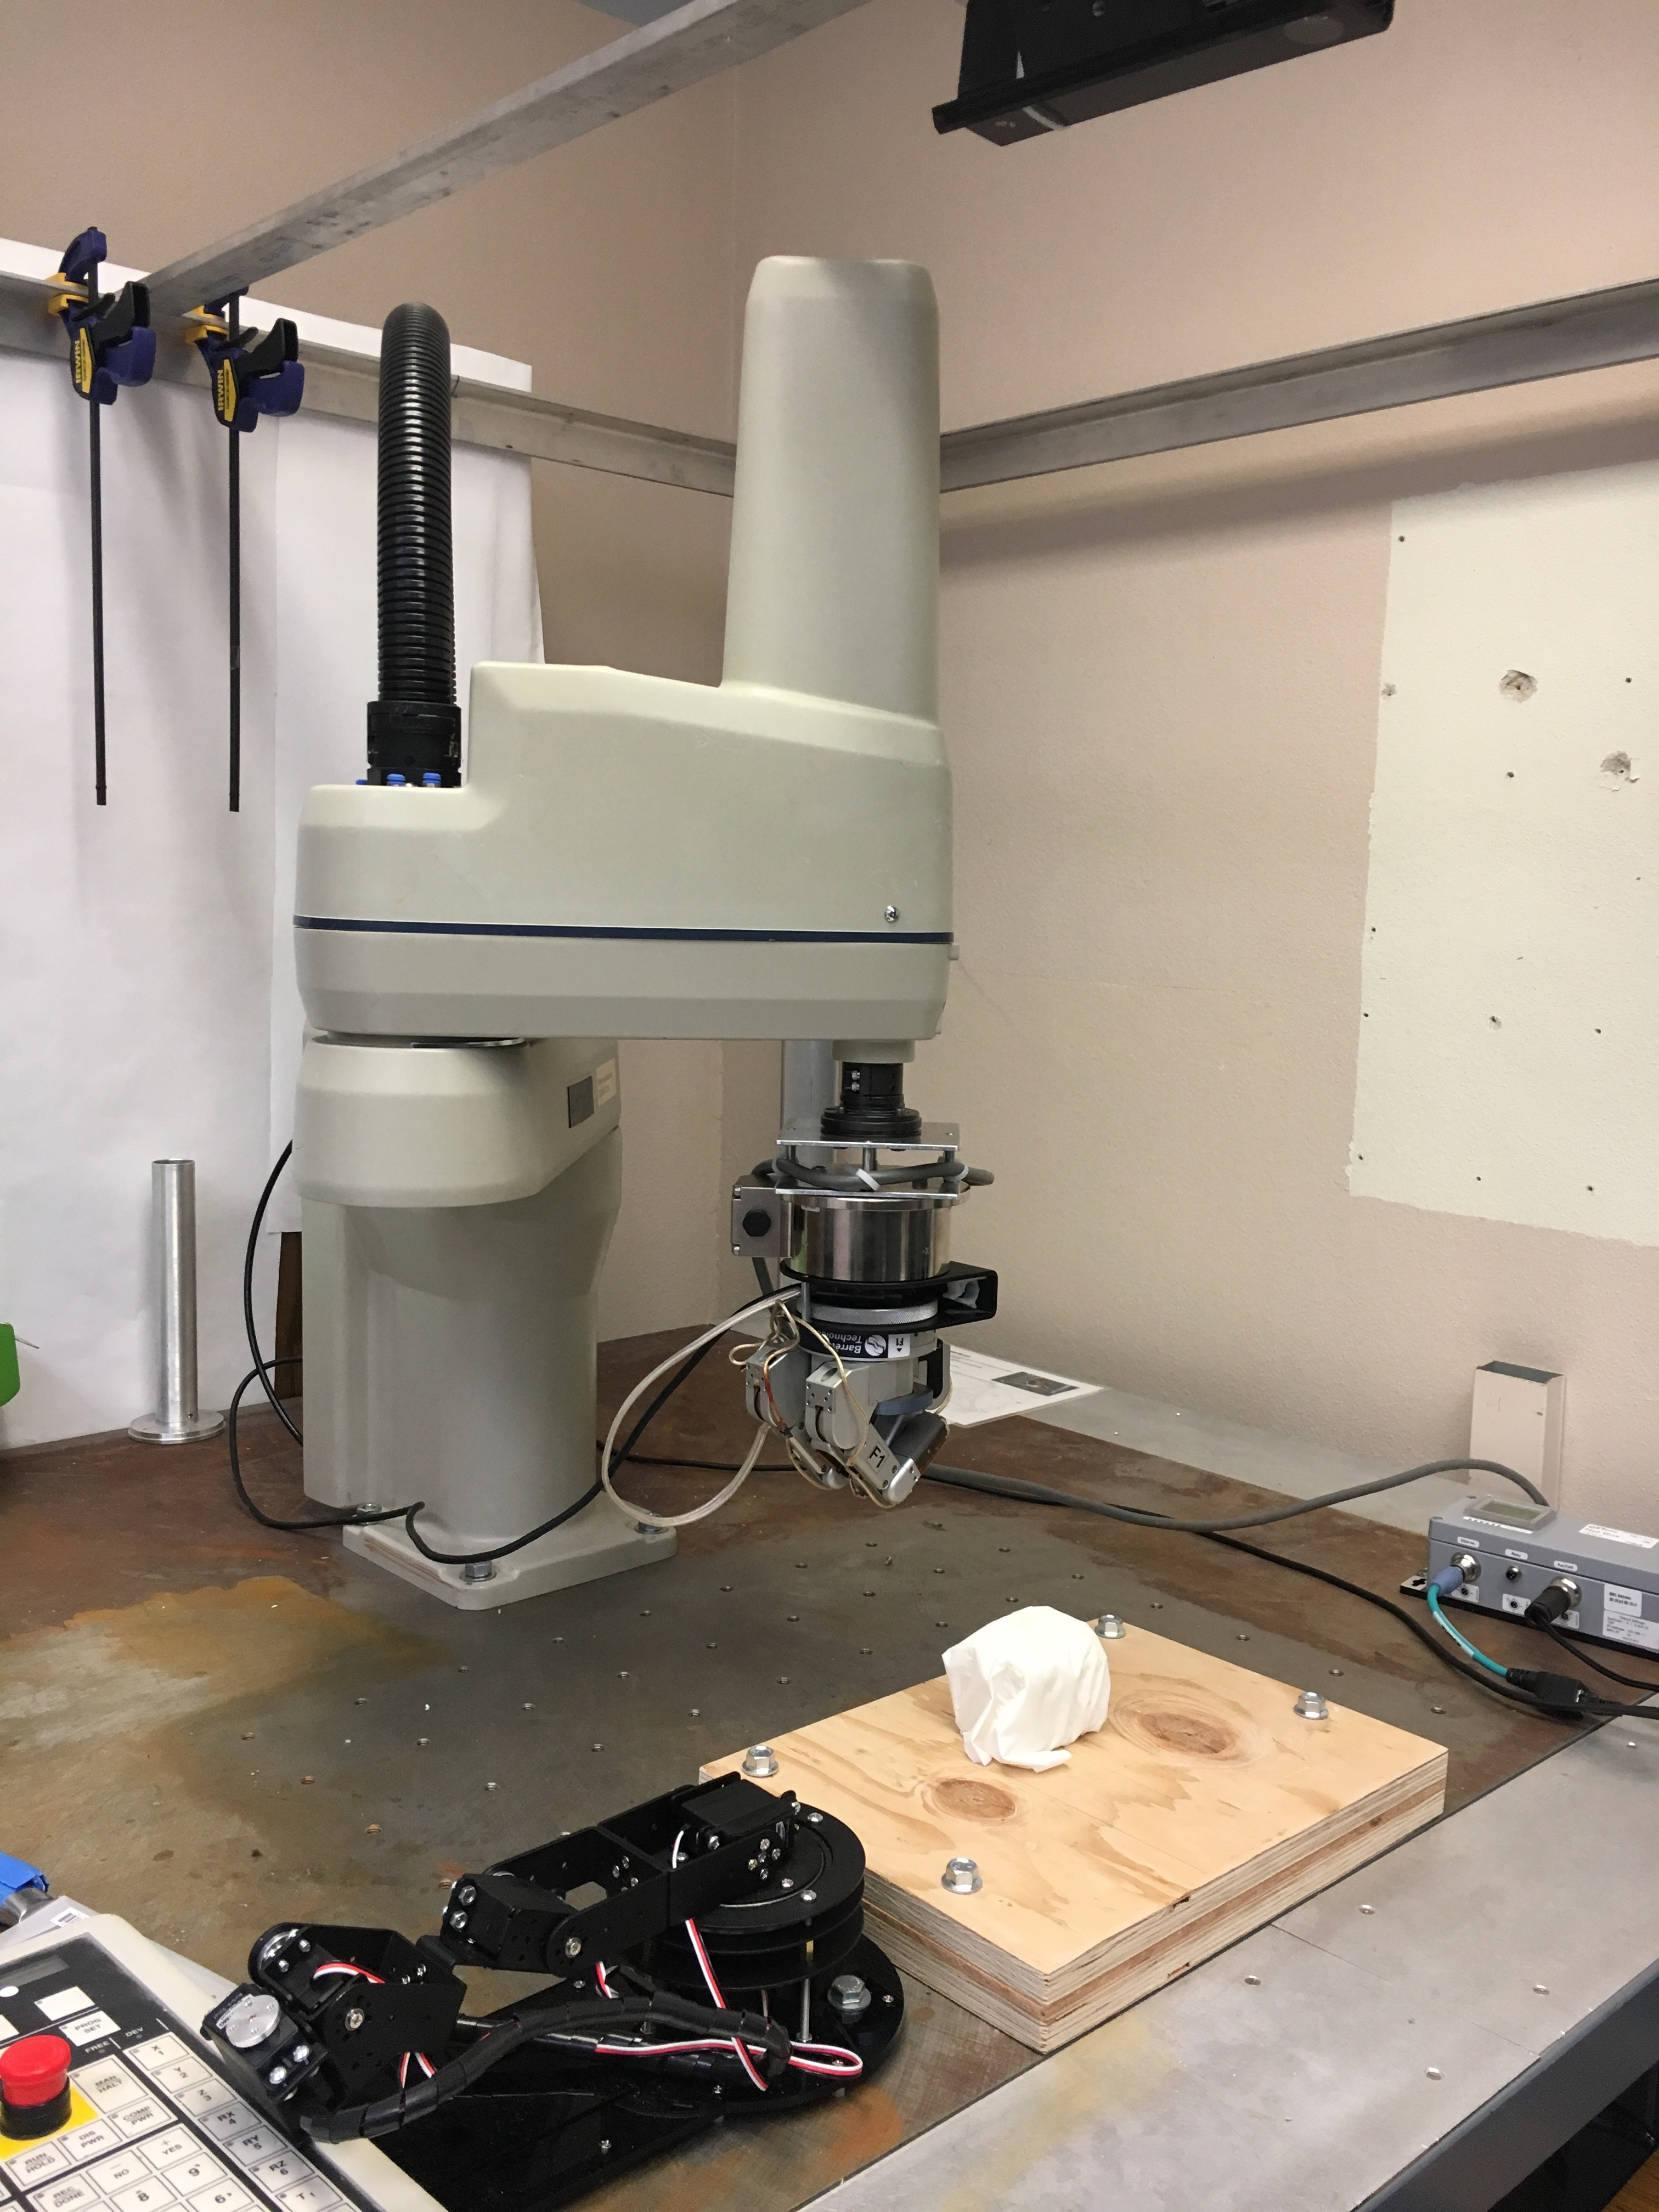
\includegraphics[width=4cm, height=5cm]{IMG_5860.jpg}
\end{frame}

\begin{frame}[fragile]{Forward Kinematics}
Known position of one point in the local frame $\pb_l$ and the current robot configuration, calculate the position of the point in the world frame Robot configuration $\pb_w$\\
\[
\begin{split}
\pb_w &=\Tb * \pb_l \\
&= \Tb_0^1 * \Tb_1^2* ... \Tb_{n-1}^n * \pb_l 
\end{split}
\]
Transformation Matrix:
\[
\Tb_{i-1}^{i}=
 \left[
 \begin{matrix}
   r_{11} & r_{12} & r_{13} & d_1\\
   r_{21} & r_{22} & r_{23} & d_2 \\
   r_{31} & r_{32} & r_{33} & d_3 \\
   0& 0 & 0 & 1
  \end{matrix}
  \right] 
\]
\end{frame}

\begin{frame}[fragile]{Inverse Kinematics}
Given a position in the world frame $\pb_w$, calculate the robot configuration under which the end-effector of the robot $\pb_l$ can reach the desired position. \\ 

From  $\pb_w =\Tb_0^1 * \Tb_1^2* ... \Tb_{n-1}^n * \pb_l$, we can know that it impossible to calculate the inverse matrix for each $\Tb_{i-1}^{i}$. 

\end{frame}



\begin{frame}[fragile] {Problem Description} 

Objective: Minimize the distance between the destination points and the lower links of the fingers�\\
	
Constraints:
\begin{itemize}
\item Limits of the rotation angles and link length of each joint(work space of the  robot)
\item	The destination points should be  on the lower link of the fingers
\item	The lower links should be perpendicular to the normal direction of the tangential plane for the destination point
\end{itemize}
	
\end{frame}



\begin{frame}[fragile] {Problem Formulation} 
\[
\min \ \  \sum_{i=0}^{2} \frac{\|(\pb_1-\qb_{11})\times (\pb_1-\qb_{12}) \|}{\|\qb_1-\qb_{12}\|}
\]

Subject to 
\[
\nb_i \times \lb_\bot =0
\]
\[
\nb_i * \lb_\bot \geq 0
\]
\[
 t_i* \qb_{i1} +(1-t_i) * \qb_{i2} = \pb_i
\]
\[
lb_i \leq \theta_i \leq ub_i  \ \ \ \     i=0, 1, ..., 7
\]
\[
0 \leq t_i  \leq 1    \ \ \ \     i=0, 1, 2
\]

\end{frame}

\begin{frame}[fragile]{Introduction}
\begin{columns}
\begin{column}{0.5\textwidth}
In constrained optimization, the general aim is to transform the problem into an easier subproblem that can then be solved and used as the basis of an iterative process.

\vspace{0.1in}

Some early methods translate the constrained problem to a basic unconstrained problem by using a \textbf{penalty function} for constraints  that are near or beyond the constraint boundary. (Interior Point Method)
\end{column}
\begin{column}{0.5\textwidth}  %%<--- here
    \begin{center}
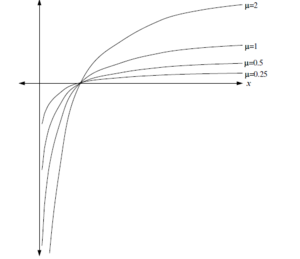
\includegraphics[width=4cm, height=5cm]{interior-point-method.png}
     \end{center}
\end{column}
\end{columns}
\end{frame}

\begin{frame}[fragile]{Introduction}
These methods are now considered relatively inefficient and have been replaced by methods that have focused on the solution of the KKT equations.

The KKT are necessary conditions for optimality for a constrained optimization problem. It is both necessary and sufficient for a global optimal point in a convex programming problem. 
\end{frame}

\begin{frame}[fragile]{Sequential Quadratic Programming}
A series of algorithms attempt to compute the Lagrange multipliers directly.

Constrained quasi-Newton methods guarantee super-linear convergence by accumulating second-order information regarding the KKT equations using a quasi-Newton updating procedure.

A quadratic programming (QP) problem will be solved at each major iteration.
\end{frame}


\begin{frame}[fragile]{Sequential Quadratic Programming}
Principal idea: \textbf{Formulate a QP subproblem based on a quadratic approximation of the Lagrangian function.}
$$L(x, \lambda) = f(x) + \sum_{i=1}^m \lambda_i \cdot g_i(x)$$

At each major iteration, an approximation is made of the Hessian of Lagrangian function. The constraints are approximated linearly. 

The solution of QP subproblem will be used to form a search direction for a line search procedure.
\end{frame}

\begin{frame}[fragile]{Sequential Quadratic Programming}
QP SubProblem:
$$ \min {1 \over 2} d^\top H_k d + \nabla f(x_k)^\top d$$
\begin{eqnarray*}
	\nabla g_i(x_k)^\top d + g_i(x_k) & = & 0, i = 1,\cdots, m_e \\
	\nabla g_i(x_k)^\top d + g_i(x_k) & \leq & 0, i = m_e+1,\cdots, m
\end{eqnarray*}
\end{frame}

\begin{frame}[fragile]{Sequential Quadratic Programming}
The SQP implementation consists of three main stages:
\begin{itemize}
  \item Updating the Hessian Matrix
  \item Quadratic Programming Solution
  \item Line Search and Merit Function
\end{itemize}
\end{frame}

\begin{frame}[fragile]{Updating the Hessian Matrix}
At each major iteration, a positive definite quasi-Newton approximation of the Hessian of Lagrangian function, $H$, is calculated using the \textbf{BFGS} method, where $\lambda_i, i = 1\cdots m$, is an estimate of the Lagrange
$$C_k^{\rm BFGS} = {q_kq_k^\top \over q_k^T s_k} - {H_k p_k p_k^\top H_k^\top \over p_k^\top H_k p_k}$$
$$H_{k+1} = H_{k} + C_k^{\rm BFGS}$$
\end{frame}

\begin{frame}[fragile]{Quadratic Programming Solution}
At each major iteraion, a QP problem of the following form is solved
$$\min {1 \over 2} d^\top H_k d + c^\top d$$
\begin{eqnarray*}
A_i d = b_i, \quad i = 1,\cdots , m_e \\
A_i d = b_i, \quad i \leq m_e + 1,\cdots , m
\end{eqnarray*}
\end{frame}

\begin{frame}[fragile]{Quadratic Programming Initialization}
    The algorithm requires a feasible point to start. If the current point from SQP method is not feasible, then we can find a point by solving the linear programming problem.
    
    $$\min \gamma$$
    such that 
    \begin{eqnarray*}
    	\Ab_i \xb & = & \bb_i, i = 1, \cdots , m_e \\
    	\Ab_i \xb  - \gamma & \leq & \bb_i, i = m_e + 1, \cdots , m
    \end{eqnarray*}
\end{frame}

\begin{frame}[fragile]{Line Search and Merit Function}
The solution to the QP subproblem produces a vector $d_k$, which is used to form a new iterate
$$\boldsymbol{x}_{k+1} = \boldsymbol{x}_k + \alpha \boldsymbol{d}_k$$
The step length parameter $\alpha_k$ is determined in order to produce a sufficient decrease in a \textbf{merit function}. 

Merit Function:
$$\Psi = f(x) + \sum_{i = 1}^{m_e} r_i \cdot g_i(x) + \sum_{i = m_e + 1}^{m} r_i \cdot \max [0, g_i(x)]$$
where $r_i$ is a penalty parameter.
\end{frame}

\begin{frame}[fragile]{Result}
    \begin{center}
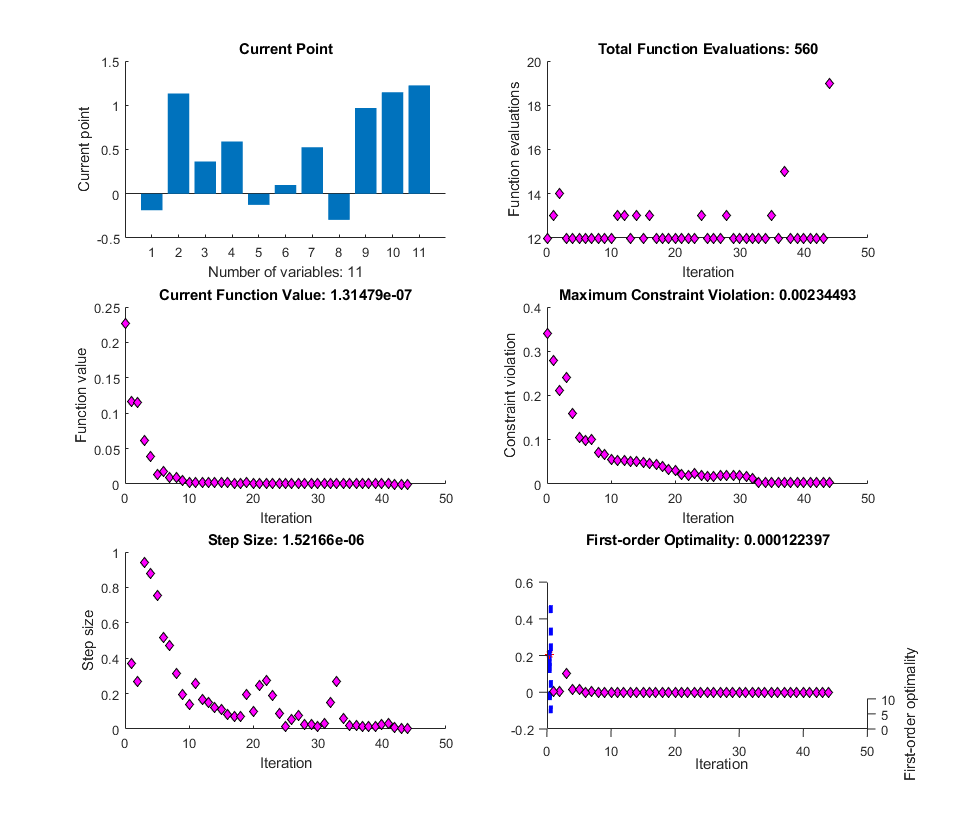
\includegraphics[width=8cm, height=8cm]{reult.png}
     \end{center}
\end{frame}

\end{document}